%Methodenwahl % Begründung der Auswahl

Industrieroboter können eine Vielzahl von verschiedenen Aufgabengebieten übernehmen. Die Aufgabengebiete reichen hierbei von Bedinungs- über Bearbeitungs- bis hin zu Montageabläufen \cite{industrieroboter_2020}. Die Schwierigkeit besteht hierbei zunächst die Anforderungen an den erforderlichen Industrieroboter zu definieren und wenn möglich einzugrenzen. Da die Kommunikation mit und ohne ROS getestet werden soll ist es von Vorteil einen Industrieroboter mit einer bereits vorhandenen ROS-Unterstützung zu verwenden. Zudem ist es erforderlich den Industrieroboter über eine direkte Schnittstelle ansprechen zu können um die gewünschten Abläufe, welche geteacht werden sollen, mit einer direkten Kommunikation ohne Netzwerklatenzen testen und einen Vergleich auf Grund des Zeitverhaltens anstellen zu können. Die Interoperabilität mit Simulationsumgebungen ist auch abzuwägen, da die Tests mithilfe einer Simulationsumgebung ohne Sicherheitsbedenken für die bedienende Person durchgeführt werden können und zudem für Regressionstests der Gestenerkennungssoftware praktikabel ohne einen realen Roboter durchgeführt werden können. Im weiteren Verlauf muss zudem die Entscheidung für einen Tiefensensor durchgeführt werden um eine Gestenerkennung, welche zur Steuerung des Inustrieroboters eingesetzt werden soll, realiseren zu können. Bei der Gestenerkennung steht vor allem die Ergonomie und die Sicherheit der bedienenden Person im Vordergrund. Hierbei muss unter anderem beachtet werden, dass zufällige Gesten nicht als Aktion gewertet werden, da dies ansonsten die Sicherheit der bedienenden Person negativ beinflussen kann. Bei der Programmiersprache und Programmierumgebung ist dabei darauf zu achten, dass diese zu ROS kompatibel ist, da ansonsten erheblicher Mehraufwand bei der Umsetzung entstehen würde.

\section{Industrieroboter}
Ein Industrieroboter ist ein universell einsetzbarer Bewegungsautomat, welcher im industriellen Einsatzgebiet eingesetzt wird. Zu erwähnen ist, dass Industrieroboter zumeist auf ein bestimmtes Problem zugeschnitten sind. Aus diesem Grund werden diese je nach der Positionsgenauigkeit, Tragfähigkeit, Arbeitsbereich, Arbeitsgeschwindigkeit und maximaler Reichweite unterschieden. Die maximale Reichweite ist bei ortsfesten Industrierobotern durch die Armlänge und die Freiheitsgrade begrenzt. Im Gegensatz zu ortsfesten Industrierobotern können bewegliche Industrieroboter sich zusätzlich in der Umgebung bewegen und werden daher durch die Bewegungsvorrichtung begrenzt \cite{industrieroboter_2020}.

\begin{figure}[htb]
	\centering
	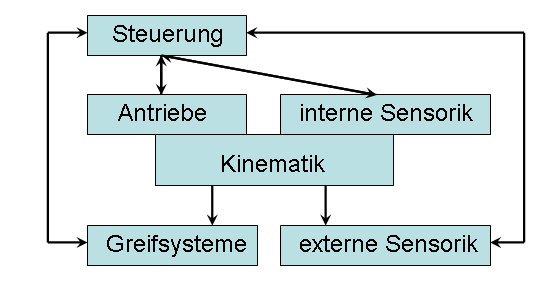
\includegraphics[width=0.6\textwidth]{images/stand_der_technik/Struktur_IR}
	\caption[Struktur eines Industrieroboters]{Struktur eines Industrieroboters \\Quelle: \cite{industrieroboter_2020}}
	\label{fig:struktur_eines_industrieroboters}
\end{figure}
\FloatBarrier

Wie in Abbildung \ref{fig:struktur_eines_industrieroboters} zu sehen ist, besteht ein Industrieroboter grundlegend aus einem Roboterarm, welcher auch Manipulator genannt wird, einer Steuerungseinheit, welche für die Überwachungung und Übersetzung der Aktionen auf den spezifischen Industrieroboter zuständig ist und einem Endeffektor, welcher über ein Greifsystem befestigt wird. Über den Manipulator, welcher Gelenke und Antriebe aufweist, wird die Kinematik realisiert, welche es ermöglicht den Manipulator im Raum zu bewegen. Um jeden Punkt im 3D-Raum ansteuern zu können sind mindestens 3 DOF erforderlich, welche über Gelenke realisiert werden. Um jeden Punkt im Raum mit jeder beliebigen Orientierung ansteuern zu können benötigt es jedoch 6 DOF, wobei 3 Gelenke für translatorische und weitere 3 Gelenke für rotatorische Bewegungsabläufe zuständig sind. Der Endeffektor kann auf verschiedene Arten realisiert werden. Zumeist ist es jedoch ein Werkzeug, welches z.B. für Schweiß-, Bohr-, Beschichtungs-, Klebe-, Montage- und Schneidearbeiten eingesetzt werden kann. Da der Endeffektor austauschbar ist, besteht jedoch aber auch die Möglichkeit einen Greifer oder einen anderen spezifisch für eine Aufgabe konzipierten Endeffektor zu montieren und zu verwenden. Damit die Steuerungseinheit die Gelenkpositionen und Antriebsgeschwindigkeiten ermitteln kann sind zudem Messsysteme erforderlich, welche als interne Sensoren bezeichnet werden. Als optionale Komponente können zudem externe Sensoren beim Industrieroboter verbaut sein, welche unter anderem zur Ermittlung von Objektposition im 3D-Raum und deren Größe verwendet werden können. Je nach Arbeitsumfeld kann es auch erforderlich sein, dass ein System zum Wechseln der Endeffektoren eingesetzt wird um mehrere Arbeitsschritte mit einem einzigen Industrieroboter durchführen zu können \cite{hagele_aufbau_2006}.

\subsection{Bauformen}
Industrieroboter können entweder zur seriellen oder parallelen Kinematik zugeordnet werden. Der Unterschied besteht darin, dass die Achsen bei der seriellen Kinematik seriell angeordnet sind, wohingegen bei der paralleln Kinematik die Achsen parallel angeordnet werden.

\begin{figure}[htb]
	\centering
	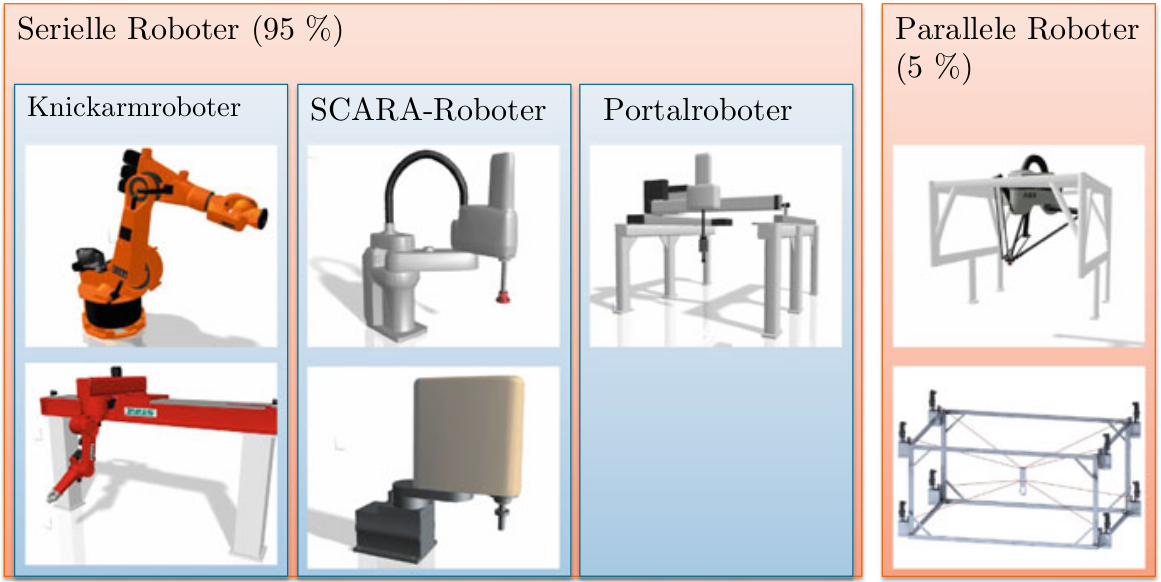
\includegraphics[width=0.9\textwidth]{images/stand_der_technik/bauformen_industrieroboter}
	\caption[Bauformen von Industrierobotern]{Bauformen von Industrierobotern \\Quelle: \cite[18]{pott_industrielle_2019}}
	\label{fig:bauformen_industrieroboter}
\end{figure}
\FloatBarrier

Mit 95\% Anteil haben sich Industieroboter mt serieller Kinematik aufgrund ihrer Bauweise und den bei Knickarmrobotern sehr großen Bewegungsfreiheit durchgesetzt, wie aus der Abbildung \ref{fig:bauformen_industrieroboter} zu entnehmen ist. Nur ein geringer Teil von 5\% der Industrieroboter besitzen eine parallele Kinematik, zu denen unter anderem der Delta- und Seil-Roboter zählen. In der Abbildung \ref{fig:bauformen_industrieroboter} ist der Delta-Roboter im Bereich der parallen Roboter oben und der Seilroboter im unteren Bereich zu sehen. Die parallele Kinematik zeichnet sich dabei durch mindestens eine geschlossene kinematische Kette aus. Zu den seriellen Industrierobotern zählen unter anderem Knick-, SCARA- und Portal-Roboter und alle anderen Roboter, welche eine offene kinematische Kette aufweisen. Industieroboter mit serieller Kinematik zählen zu den am weitest verbreitesten Industrierobotern. Im Gegensatz zu den seriellen Industrierobotern bieten parallele Industrieroboter durch die direkte Verbindung zum Greifsystem den Vorteil, dass die nachfolgenden Glieder und deren Massen nicht wie beim seriellen Industrieroboter die Dynamik des Systems beeinflussen. Dies führt dazu, dass eine sehr hohe Genauigkeit und eine sehr hohe Steifigkeit garantiert werden kann. Zudem sind durch die parallele Kinematik hochpräzise Ansteuerungsmanöver mit sehr hoher Geschwindigkeit durchführbar. Der Nachteil besteht jedoch darin, dass der parallele Industrieroboter ortsfest ist. Die parallele Kinematik zählt daher eher zur Ausnahme und wird aus diesem Grund vermehrt für Pick-and-Place-Aufgaben oder Sondermaschinen eingesetzt, wo Geschwindigkeit, eine hohe Präzision und hohe Dynamik erforderlich ist \cite[17\psqq]{pott_industrielle_2019}.\\

Der Knickarmroboter, welcher zu den seriellen Industrierobotern zählt und zumeist 6 DOF aufweist, bietet den Vorteil, dass dieser für weitere Bewegungsfreiheit auf eine zusätzliche Linearachse montiert werden kann. Dadurch ist es unter anderem Möglich verschiedene Arbeitspositionen eines großen Objekts ansteuern zu können. Da der Knickarmroboter eine armartige Form aufweist, ist dieser zumeist für schwer erreichbare Stellen geeignet. Aufgrund der offenen kinematischen Kette und der Möglichkeit einer sehr großen Nutzlast leidet jedoch die Absolutgenauigkeit darunter. Typischwerweise werden Knickarmroboter für Schweiß-, Handhabungs- und Klebearbeiten eingesetzt. Eine weitere Möglichkeit um serielle Industrieroboter zu realisieren stellen die SCARA-Roboter dar. Diese weisen im Gegensatz zu den Knickarmrobotern weniger Freiheitsgrad. Typischwerweise werden zumeist 3 oder 4 DOF verbaut, wodurch die Bewegungsfreiheit eingeschänkt wird. Zudem sind aufgrund der Bauform nur geringere Arbeitslasten und kleinere Arbeitsbereiche nutzbar. Dies zeigt sich auch beim Aufgabenbereich, welcher großteils in der Montage und Pick-and-Place besteht. Portale, welche auch zu den seriellen Industrierobotern zählen, können sehr hohe Nutzlasten und große Bewegungen durchführen. Sie sind nach den Knickarmrobotern die zweithäufigste Bauform. Zu den Aufgabengebieten zählen Pick-and-Place, Maschinenbestückungen und Kommisionsarbeiten \cite[17\psqq]{pott_industrielle_2019}.

\subsection{Positions- und Bahngenauigkeit}
Um Genauigkeitsmessungen an einem Industrieroboter durchzuführen ist es erforderlich die spezifischen Genauigkeiten eines Industrieroboters zu kennen und diese in einen Zusammenhang zu bringen. Bei Industrierobotern ist die Genauigkeit in sehr vielen Aufgabenbereichen, wie z.B Laserschneiden oder Schweißen, sehr entscheident. Eine hohe Genauigkeit spart Kosten und Zeit ein, da eine teure und zeitintensive Nachbearbeitung entfällt. Aus diesem Grund ist es entscheident, dass der Industieroboter für spezielle Aufgabenbereiche eine hohe Positions- und Bahngenauigkeit aufweist. Um die Positions- und Bahngenauigkeit von Industrierobotern beurteilen zu können verwendet man die Absolut- und Wiederholgenauigkeit. Beide Kennwerte beschreiben die Qualität der Übereinstimmung der Realität und des Modells und sind in der ISO 9283, welche die Robotergenauigkeit beinhaltet und beschreibt, standardisiert \cite[28\psqq]{pott_industrielle_2019}.

\begin{figure}[htb]
	\centering
	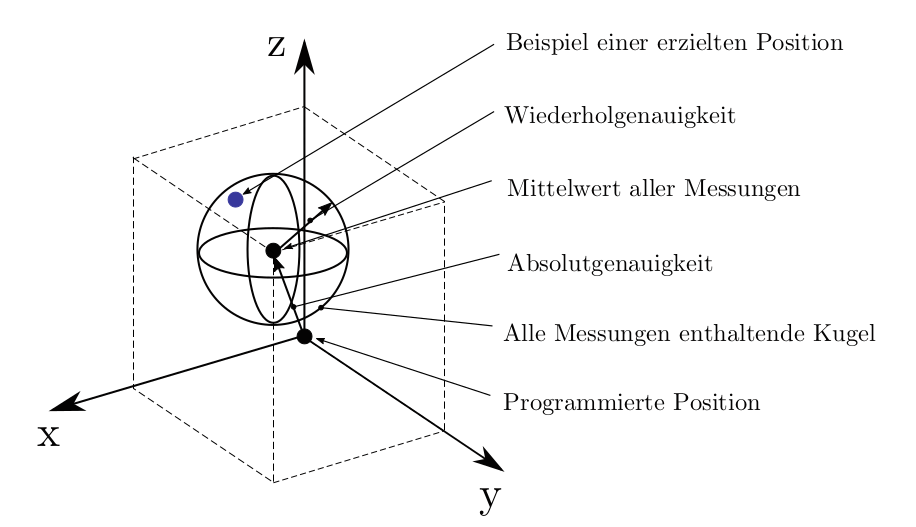
\includegraphics[width=0.686\textwidth]{images/stand_der_technik/absolutgenauigkeit_und_wiederholgenauigkeit}
	\caption[Absolut- und Wiederholgenauigkeit]{Absolut- und Wiederholgenauigkeit \\Quelle: \cite[29]{pott_industrielle_2019}}
	\label{fig:absolutgenauigkeit_und_wiederholgenauigkeit}
\end{figure}
\FloatBarrier

In der Abbildung \ref{fig:absolutgenauigkeit_und_wiederholgenauigkeit} ist der Zusammenhang zwischen der Absolut- und Wiederholgenauigkeit zu erkennen. Die Wiederholgenauigkeit wird ermittelt indem der Industrieroboter über mehrere Zyklen hinweg immer wieder die gleiche Pose aus einer spezifischen Richtung anfährt und am Ende die dabei entstandenen Abweichungen gemittelt werden. Hierbei beeinflussen systematische Gegebenheiten, wie z.B. termische Ausdehnung durch Umgebungstemperatur, sowie aber auch durch die Motorwärme, Justagefehler der Achsen, Fertigungstoleranzen oder sogar Kollisionen die Genauigkeit des Gesamtsystems um die Zielpose exakt ansteuern zu können. Aus diesen Gründen ist es empfehlenswert den Industrieroboter jährlich auf die Genauigkeit zu prüfen und gegebenenfalls zu justieren. Im Gegensatz zur Wiederholgenauigkeit beschreibt die Absolutgenauigkeit wie genau der Industrieroboter eine theoretisch programmierte Zielpose, z.B. mittels CAD-Software erlernt, im Bezug zum Roboterkoordinatensystem im Durchschnitt aus einer beliebigen Richtung ansteuern kann. Standardmäßig beträgt die Wiederholgenauigkeit bei Industrierobotern \num{0,1} mm wohingegen die Absolutgenauigkeit standardmäßig eine maximale Abweichung von 1 mm aufweist \cite[28\psqq]{pott_industrielle_2019}.

\begin{figure}[htb]
	\centering
	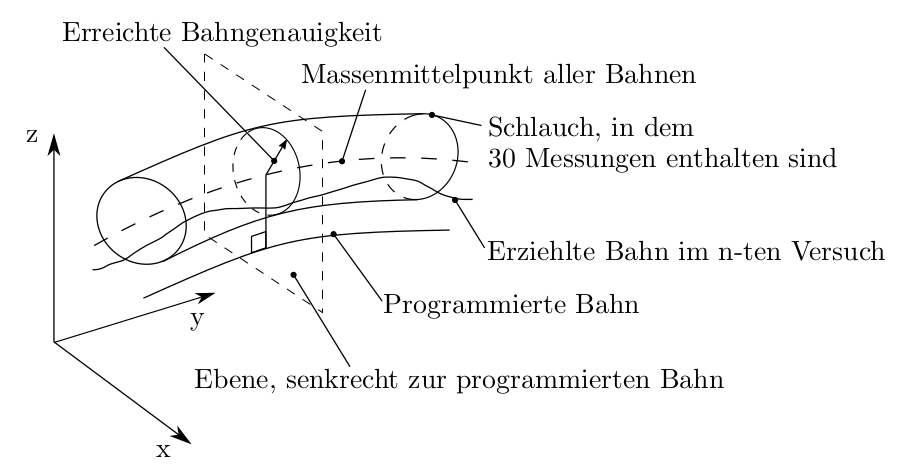
\includegraphics[width=0.735\textwidth]{images/stand_der_technik/bahngenauigkeit}
	\caption[Bahngenauigkeit]{Bahngenauigkeit \\Quelle: \cite[30]{pott_industrielle_2019}}
	\label{fig:bahngenauigkeit}
\end{figure}
\FloatBarrier

Bei einer großen Abweichung der Absolutgenauigkeit führt dies jedoch zu einem schlechten erreichen der Zielpose und dadurch auch zu einem schlechten Bahnverhalten wie in Abbildung \ref{fig:bahngenauigkeit} durch die erzielte Bahn im n-ten Versuch ersichtlich ist. Die erzielte Bahn weist deutliche Schwingungen auf und weicht daher erkennbar von der programmierten Bahn ab. Aus diesem Grund bieten viele Hersteller gegen einen Aufpreis absolutvermessene Industrieroboter an um diesen Genauigkeitsfehler zu kompensieren \cite[29\psq]{pott_industrielle_2019}. Wenn eine sehr hohe Wiederholgenauigkeit gewünscht ist kann auch mit Spezialrobotern eine Wiederholgenauigkeit von bis zu 1 \si{\micro}m erreicht werden \cite{genauigkeit_nodate}.

\begin{figure}[htb]
	\centering
	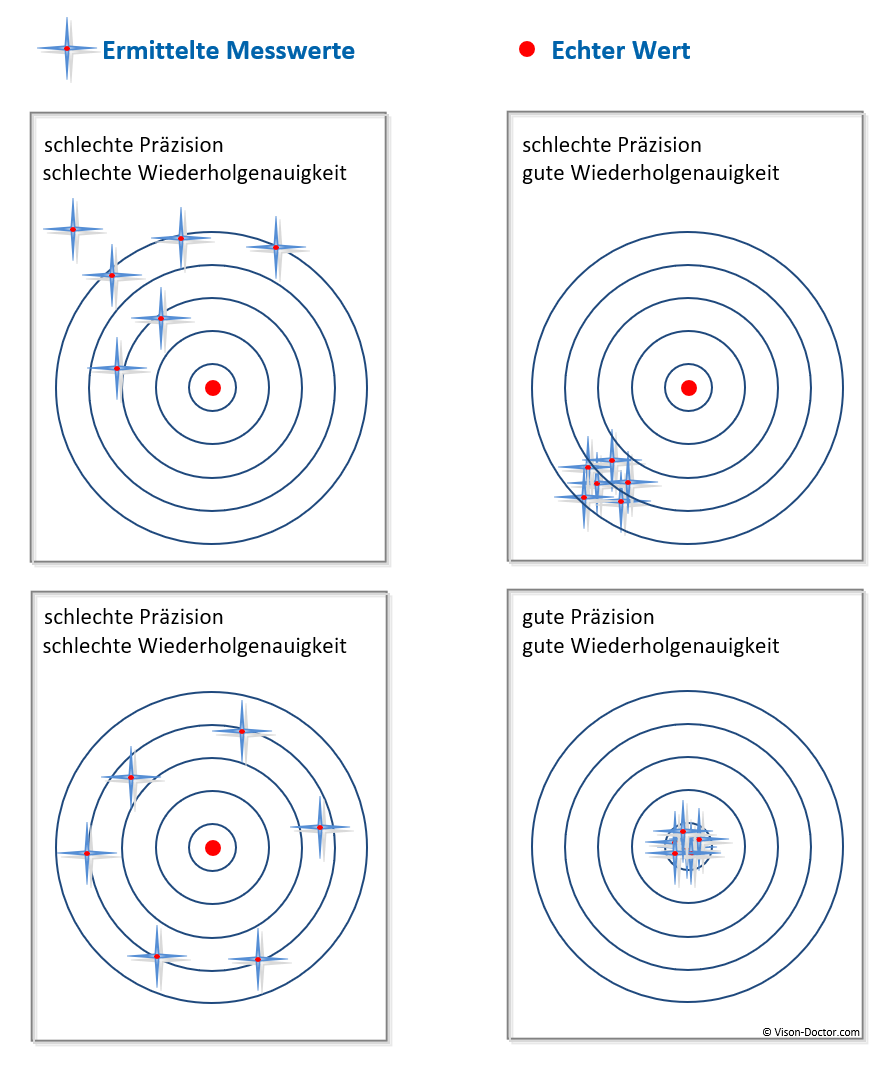
\includegraphics[width=0.57\textwidth]{images/stand_der_technik/wiederholgenauigkeit}
	\caption[Wiederholgenauigkeit]{Wiederholgenauigkeit \\Quelle: \cite{prazision_nodate}}
	\label{fig:wiederholgenauigkeit}
\end{figure}
\FloatBarrier

Wie in Abbildung \ref{fig:wiederholgenauigkeit} zu sehen ist, kann daraus geschlossen werden, dass keine hohe Präzision durch eine schlechte Wiederholgenauigkeit möglich ist. Aus diesem Grund kann auch gesagt werden, dass die Wiederholgenauigkeit entscheidenter als die Absolutgenauigkeit zum erreichen der Zielposition ist, da umgekehrt nicht gesagt werden kann, dass eine hohe Präzision durch eine gute Wiederholgenauigkeit erreicht wird \cite{genauigkeit_nodate}.


%"Die genaue Definition findest Du in der EN ISO 29283 (ehemals ISO 9283). Dort wird auch beschrieben, wie man die Genauigkeiten ermittelt." (https://www.roboternetz.de/community/threads/35643-absolutgenauigkeit)



% ----------------------

% S. 25 pott_industrielle_2019   kinematische Transformation (direkte & indirekte Transformation)
% cBei seriellen Robotern ist die direkte Kinema- tik stets eindeutig, während es für eine gewünschte Position des Endeffektors häufig mehr als eine Lösung gibt. Bei Knickarmrobotern kann es je nach Position bis zu acht mögliche Achsstellungen für eine vorgegebene Position des Endeffektors geben.``



% S. 54 - 56 pott_industrielle_2019

%\subsection{Bewegungsdynamik}
%\subsection{Steifigkeit}




% https://www.youtube.com/watch?v=wKiJaK-RDKI
% https://www.youtube.com/watch?v=GNrU2zviRpc
% https://www.youtube.com/watch?v=A9M1zX3GzX0
% https://www.youtube.com/watch?v=9iCLK__7ymY



% https://de.wikipedia.org/wiki/Industrieroboter
% https://link.springer.com/chapter/10.1007%2F3-540-34823-9_27

% Wie schnell können diese reagieren? (Zeitverhalten) je nach Roboterarm verschieden


\section{Teachen von Industrierobotern}
Teachen, welches auch als Teach-In bezeichnet wird, ist eine von mehreren möglichen Varianten einem Industrieroboter gewünschte Posen beizubringen, damit dieser seine Arbeitsaufgabe autonom durchführen kann.

\subsection{Offline- und Online-Programmierverfahren}
Unterschieden wird bei den Lernmethoden zwischen Offline- und Online-Programmierverfahren. Die am weitest verbreitesten Offline-Methoden sind die textuelle Programmierung und das Erlernen mit einer CAD-Software. Bei der textuellen Programmierung ist es notwendig über ausreichend Programmierkenntnisse in der Programmiersprache des Industieroboter-Herstellers oder einer kompatiblen Programmiersprache zu verfügen, wohingegen bei einer CAD-Software einem virtuellen Industrieroboter in einer virtuellen Umgebung die Posen beigebracht werden können. Beide Methoden benötigen im Vergleich zum Teachen sehr viel mehr Vorwissen und sind daher nur nach erheblichem Lernaufwand nutzbar. Das Teachen zählt neben der Playback-Methode, welches ein direktes Führen des Roboterarms ermöglicht, zu den Online-Programmierverfahren. Beim Teachen kommt eine Steuerkonsole zum Einsatz mit deren Hilfe es möglich ist dem Industieroboter Posen beizubringen. Zuerst wird eine Pose mit mehreren aufeinander folgenden Steuerungsbefehlen angefahren. Anschließend, wenn eine gewünschte Pose erreicht wurde, kann diese einzelne Pose per Steuerungsbefehl in der Steuerungseinheit gespeichert werden. Das Anfahren und Speichern der Posen wird solange wiederholt bis die gesamte Arbeitsaufgabe dem Industrieroboter beigebracht wurde. Wenn notwendig, können im Nachhinein die gespeicherten Posen korrigiert werden um eine höhere Genauigkeit zu erzielen oder um Fehler zu korrigieren. Im Gegensatz zum Teachen wird beim Playback-Verfahren genau die Bewegung gespeichert, welche durch das direkte Führen des Roboterarms entsteht, und beim Ausführen der Arbeitsaufgabe auf die gleiche Weise wiederholt \cite{industrieroboter_2020}. Beim Teachen hingegen kann zwischen den Punkten die Geschwindigkeit, Beschleunigung und sogar die Art des Pfades eingestellt werden. Bei der Art des Pfades kann frei zwischen Point-to-Point und Continuous Path gewählt werden. Point-to-Point erzwingt den für den Industrieroboter geometrisch günstigsten Pfad zwischen den Punkten zu wählen, welcher normalerweise keine gerade lineare Bahnbewegung darstellt und daher zu einem unbekannten Pfad führt. Bei Continuous Path wird hingegen von einem Punkt direkt zum nächsten Punkt entlang eines vordefinierten Pfades gefahren, welcher z.B. eine gerade lineare oder eine durch einen Hilfspunkt erzeugte kreisförmige Bahnbewegung sein kann. Durch diese Einstellungsmöglichkeiten ist es beim Teachen möglich noch höhere Genauigkeiten als bei der Playback-Methode zu erzielen. Im Gegenzug steigt durch die höhere Genauigkeit, aber auch der Programmieraufwand, da für eine hohe Genauigkeit viele Zwischenpunkte gelernt werden müssen \cite{teach-technik_2020}.\\

Für alle Programmierverfahren, ob Offline- oder Online-Programmierverfahren, welche zur Programmierung von Industrierobotern eingesetzt werden, kann gesagt werden, dass sie einen gewissen Lernaufwand bei der Einarbeitung benötigen. Der Lernaufwand um ein Programmierverfahren zu erlernen sinkt jedoch erheblich für untrainierte Personen, wenn eine visuelle Lernmethode eingesetzt wird. In Zukunft besteht daher ein sehr großes Potenzial zur Erforschung und Verbesserung von Gesten, Sprach und visuellen Systemen, da diese Systeme eine für den Menschen vertrauliche Interaktionsmöglichkeit bieten \cite{biggs_survey_nodate}.\clearpage

\subsection{Teach Pendant}
\begin{figure}[htb]
	\centering
	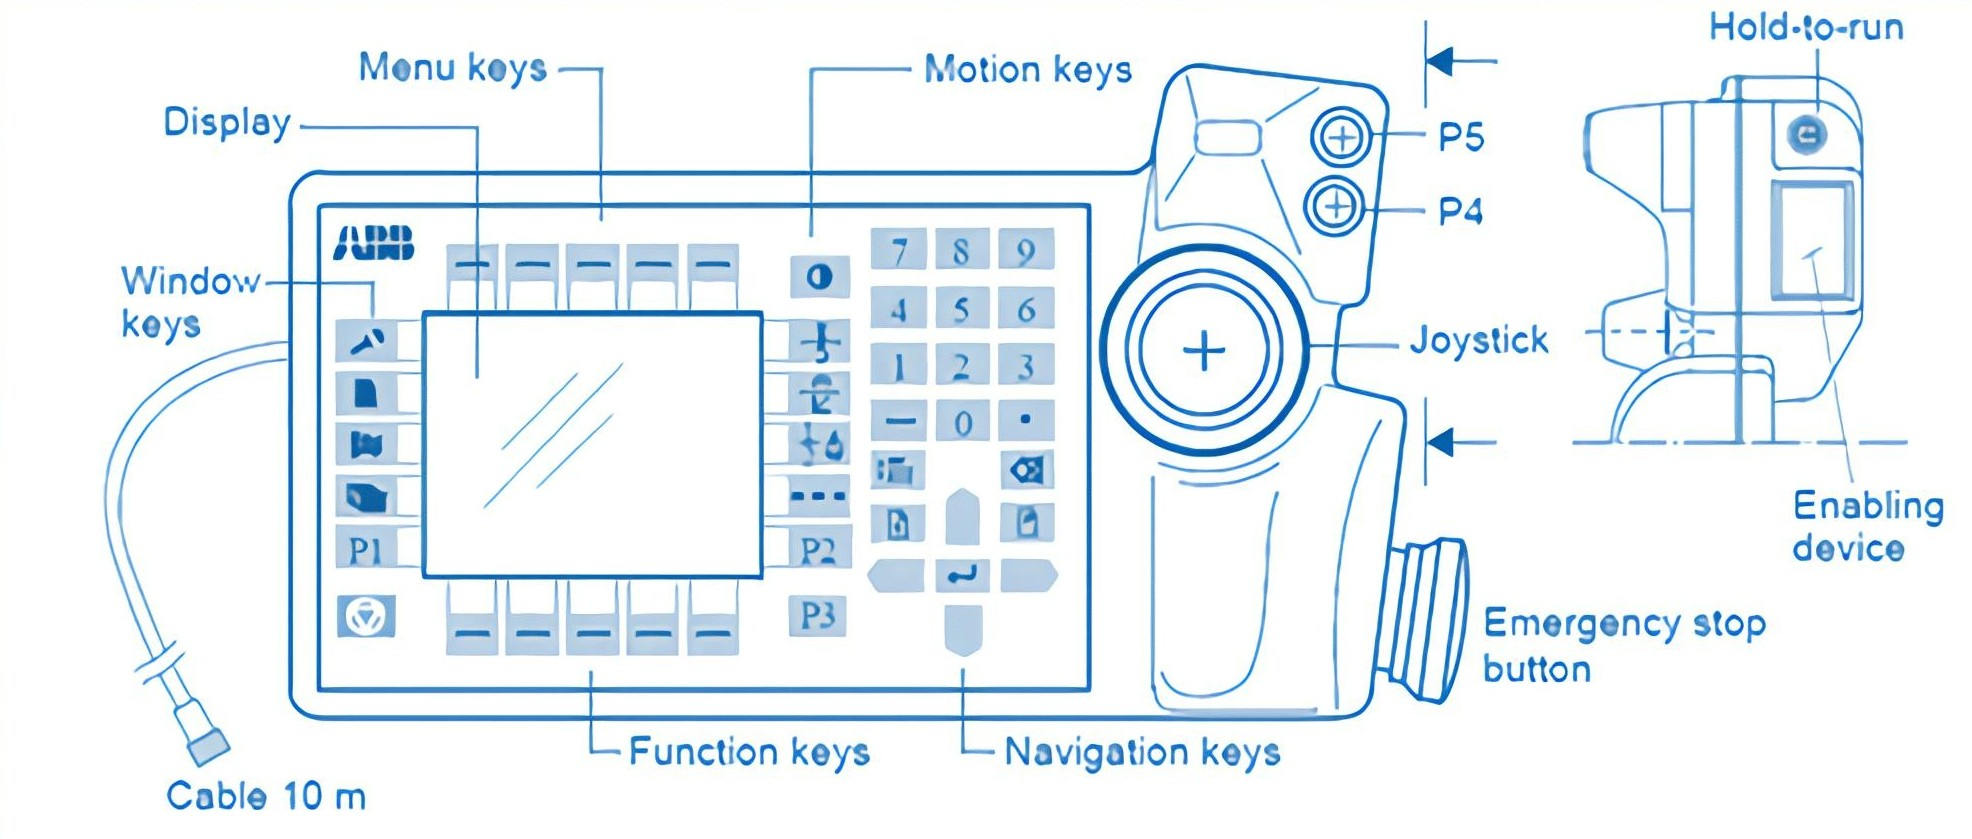
\includegraphics[width=0.715\textwidth]{images/stand_der_technik/teach_pendant}
	\caption[Teach Pendant im Querformat von ABB]{Teach Pendant im Querformat von ABB \\Quelle: \cite{programengif_nodate}}
	\label{fig:teach_pendant}
\end{figure}
\FloatBarrier

Zur Programmierung mit dem Teach-In-Verfahren werden Teach Pendants, wie in Abbildung \ref{fig:teach_pendant} zu sehen, eingesetzt, welche im Gegensatz zu früheren Modellen je nach Hoch- oder Querformat im oberen oder im linken Bereich des Teach Pendants über ein Display mit oder ohne Touch-Funktionalität verfügen \cite{nof_handbook_1999}. Unterschieden wird bei den herstellerspezifischen Teach Pendants zwischen dem Hoch- und Querformat. Beim Hochformat wird das Teachpendant mit beiden Händen gehalten und mithilfe der Daumen werden die Knöpfe betätigt. Im Gegensatz zum Hochformat ist in einem Teach Pendant mit Querformat ein größeres Display verbaut und das Teach Pendant kann im Querformat mit beiden Händen oder nur mit der linken Hand gehalten werden. Die rechte Hand kann dazu verwendet werden Eingaben auf dem Teach Pendant zu tätigen oder mittels des verfügbaren 3 DOF Joysticks oder 6 DOF 3D-Maus zum Steuern des Industrieroboters verwendet werden. Beim Betätigen des Joysticks oder der 3D-Maus reagiert der Industrieroboter bereits bei sehr feinen Bewegung des Eingabegerätes mit einer entsprechenden Bewegung in die jeweilige vorgegebene Richtung. Je weiter der Joystick oder die 3D-Maus in eine Richtung bewegt wird, desto schneller bewegt sich auch der Industrieroboter in die ensprechende Richtung \cite[48\psq]{prassler_advances_2004}. Jedes Teach Pendant muss einen Notstop-Schalter aufweisen um die Maschine und das Teach Pendant jederzeit außer Betrieb setzen zu können. Dieser Notstop-Schalter ist zumeist rechts oben oder rechts unten, wie in Abbildung \ref{fig:teach_pendant} zu sehen ist, als große rote Taste realisiert. Als weitere Schutzvorkehrung muss das Teach Pendant einen \quoteMark{Enable device}-Schalter aufweisen. Der \quoteMark{Enable device}-Schalter wird Umgangssprachlich auch \quoteMark{Dead Man's Switch} genannt und muss während die Maschine bedient wird ununterbrochen gehalten werden. Dabei ist zu beachten, dass wenn der Notstop-Schalter losgelassen oder zu fest gedrückt wird, der Industrieroboter zum Anhalten gebracht wird. Das Teach Pendant geht davon aus, dass wenn dieser Schalter zu fest gedrückt oder losgelassen wird, dass die Person, welche die Kontrolle über das Teach Pendant hat bewusstlos, Tod oder sogar nicht mehr an der Maschine ist. Durch das Auslösen dieses Sicherheitsschalters wird der Industrieroboter zum Anhalten gebracht und weiterer Schaden und gefährliche Situationen werden verhindert \cite{dead_man_switch_2020}.\\

Weitere Tasten wie z.B. Menü, Funktionen, Bewegung und Navigation, wie in Abbildung \ref{fig:teach_pendant} zu sehen ist, sind herstellerspezifisch und daher optional. Aus diesem Grund kann ein Teach Pendant je nach Hersteller unterschiedliche herstellerspezifischen Funktionstasten aufweisen, welche zumeist Zugriff auf die am häufigsten verwendeten Funktionalitäten des Teach Pendants bieten \cite{dinwiddie_basic_2015}. Neben diesen Sicherheitsfeatures gibt es auch herstellerübergreifende Features um den Industrieroboter zu steuern. Eines dieser Features ist das Wechseln zwischen unterschiedlichen Bewegungsmodi. Zu diesen Bewegungsmodi zählen der Gelenk-, Welt-Koordinatensystem- und Tool-Koordinatensystem-Modus. Der Gelenk-Modus erlaubt es die Position der Gelenke mithilfe des Teach Pendants jeweils einzeln oder alle Gelenke zusammen zu bewegen. Dieser Modus ermöglicht es daher die volle Kontrolle über alle Gelenke des Industrieroboters zu erlangen und diese an die jeweiligen Gegebenheiten der Umgebung anzupassen. Der Gelenk-Modus wird daher häufig zum Erreichen von schwer zugänglichen Stellen eingesetzt. Im Gegensatz zum Gelenk-Modus erlaubt es der Welt-Koordinatensystem-Modus den Mittelpunkt des Endeffektors (TCP) in der x-, y- oder z-Achse zu bewegen und Rotationen um die x-, y- oder z-Achse im Weltkoordinatensystem durchzuführen. Der Sockel des Industrieroboters stellt den Mittelpunkt des Weltkoordinatensystems dar. Für diesen Modus werden die Positionen der Gelenke über die inverse Kinematik, ermittelt und automatisch vom Teach Pendant eingestellt \cite{jogging_2017}. Wenn bei Knickarmrobotern die Pose des Endeffektors bei der Berechnung der inversen Kinematik berücksichtigt wird, kann es je nach gewählter Pose des Endeffektors bis zu acht mögliche Gelenksstellungen für den Knickarmroboter geben, wordurch die inverse Kinematik für diesen Fall nicht mehr eindeutig für die gewählte Pose ist \cite[25]{pott_industrielle_2019}. Die letzte Möglichkeit den Industrieroboter einzustellen besteht darin, den TCP des Industrieroboters im Tool-Koordinatensystem-Modus einzustellen. Der Tool-Koordinatensystem-Modus besitzt die gleichen Möglichkeiten, wie der Welt-Koordinatensystem-Modus, verwendet jedoch aber als Referenzkoordinatensystem den TCP \cite{jogging_2017}.

% Genauigkeit % TODO: Welche Genauigkeit ist mit einem Teach Pendant möglich?


% Überschleifen: https://www.xplore-dna.net/mod/page/view.php?id=451

% Robotersteuerung (Bewegungsbahn): https://wiki.induux.de/Robotersteuerung

% Point-to-point: https://www.youtube.com/watch?v=Fd7wjZDoh7g

% https://www.computerwoche.de/a/mikroprozessoren-machen-programmierung-erst-effektiv,1160823


\section{Arten von Echtzeitverhalten}
Im Umgang mit Industrierobotern ist es notwendig Echtzeitsysteme einzusetzen, welche für den jeweiligen spezifischen Anwendungsfall die Anforderung an die Reaktionszeit des Systems sicherstellen. Die Anforderung an das Echtzeitsystem können vielseitig sein. Diese können bei sehr zeitkritischen und sicherheitsrelevanten Systemem wenige Millisekunden und bei weniger relevanten Aufgaben, wie z.B. das Speichern von Daten auf eine Festplatte, bis hin zu mehreren Minuten, Stunden, Tagen oder sogar länger in Anspruch nehmen. Die entscheidente Herausforderung für das Echtzeitsystem ist es deshalb zu garantieren, dass das Ergebnis in dem für den Anwendungsfall erforderlichen Zeitintervall geliefert wird. Die möglichen Zeitintervalle werden durch die Hardware limitiert, wordurch eine für den Anwendungsfall entsprechend schnelle Hardware erforderlich ist. Anwendungsfälle mit genügend kleinen Zeitinvervallen können daher nur mit entsprechend schneller Hardware realisiert werden \cite{echtzeitsystem_2020}.

\subsection{Echtzeitanforderungen}
Bei Echtzeitsystemen wird zwischen harter, fester und weicher Echtzeitanforderung unterschieden. Unter harter Echtzeitanforderung versteht man, dass das Ergebnis innerhalb des vorgegebenen Zeitintervalls  erfolgen muss, da ansonsten das System versagt hat. Bei Nichteinhaltung des Zeitintervalls besteht ansonsten die Möglichkeit, dass es zu einem Schaden kommt. Als Beispiel kann die Notbremsung eines autonom fahrenden Autos eine harte Echtzeitbedingung darstellen. Im Gegensatz zur harten Echtzeitanforderung stellt die feste Echtzeitanforderung eine etwas gelockertere Echtzeitanforderung dar. Bei der festen Echtzeitanforderung wird davon ausgegangen, dass kein unmittelbarer Schaden zustande kommt, wenn das vorgegebene Zeitintervall überschritten wird. Daher kann das vorgegebene Zeitintervall problemlos bei der festen Echtzeitanforderung überschritten werden. Das Ergebnis wird beim Überschreiten des Zeitintervalls jedoch zumeist ungültig und weitere darauf aufbauende Berechnungen können daher abgebrochen werden. Ein Beispiel für eine feste Echtzeitanforderung kann z.B. sein, dass die derzeitige Position eines Fahrzeugs nach dem Weiterfahren nicht mehr die gleiche Position ist und Berechnungen auf diesen Daten schlicht zu falschen Ergebnissen führen würden. Aus diesem Grund würde es keinen Sinn machen mit den veralteten Daten weiterzuarbeiten. Bei weichen Echtzeitanforderung ist das Zeitintervall für die Bearbeitung der Aufgabe als Richtwerte zu sehen und kann bei der Abarbeitung der Aufgabe wenig oder sehr stark überschritten werden. Im Mittel werden die Aufgaben jedoch zeitgerecht abgearbeitet. Zum Beispiel bei Multimediasystemen führen geringe Überschreitungen des Zeitintervalls zu verzögert wiedergegebenen Bildern. In einem gewissen Rahmen sind diese Verzögerung daher akzeptabel. Ab dem Zeitpunkt ab dem das Video anfängt zu stottern und auszusetzen und die Verzögerung von Menschen wahrgenommen werden kann ist zumeist die Akzeptanzgrenze bereits weit überschritten \cite[321\psq]{worn_echtzeitsysteme_2006}.\\

Um die harte, feste oder weiche Echtzeitanforderungen auf konventionellen Computern mit mehreren Prozessen umsetzen zu können werden sogenannte Echtzeitbetriebssysteme (RTOS) eingesetzt. Bei einem Echtzeitbetriebssystem stellt der RTOS-Kernel die notwendige Komponente dar, welche die Echtzeitanforderung realisiert\cite[343\psq]{worn_echtzeitsysteme_2006}. Ein Kernel ist die grundlegene Komponente eines Betriebssystems, welche die Hardwareabstraktion, Prozessverwaltung, Speicherverwaltung und andere wiederverwendbare Ressourcen bereitstellt um die Entwicklung von Programmen zu erleichtern \cite[356]{worn_echtzeitsysteme_2006}. Im Gegensatz zu einem Betriebssystem ohne Echtzeitanforderung ist es bei einem Echtzeitbetriebssystem erforderlich, dass das Prozess-Scheduling, welches bestimmt wann und wie viel Zeit ein Prozess erhält, deterministisch abläuft, sodass die Prozesse die Ergebnisse zeitgerecht im benötigten Zeitintervall erhalten. Bei einer Echtzeitanwendung muss nicht nur der Prozess-Scheduler die Echtzeitfähigkeit unterstützen, sondern auch die Anwendung explizit die Echtzeitanforderungen beachten um vollen Gebrauch von der Echtzeitfähigkeit des Systems machen zu können. Neben dem Prozess-Scheduler können auch Ein- und Ausgaben, zu denen unter anderem das Betätigen von Tasten, die Netzwerkkommunikation und das Schreiben und Lesen von Daten von einem Speichermedium gezählt werden, die Echtzeitfähigkeit eines Systems beeinflussen. Aus diesem Grund sollte der virtuelle Speicher, welcher zum Auslagern auf die Festplatte oder SSD verwendet werden kann, deaktiviert sein um nicht-deterministisches Verhalten zu vermeiden. Für Echtzeitsysteme ist es auch erfordlich, dass der Bedarf an Ressourcen, welches den verfügbaren Arbeitsspeicher miteinschließt, bekannt ist. Zumeist wird dies erreicht indem im Vorhinein genügend Arbeitsspeicher für die Anwendung reserviert wird. Das Reservieren von Arbeitsspeicher oder Betriebssystemfunktionen aufzurufen ist ein sehr aufwändiger Prozess, welcher die Anwendung über das Zeitinvervall hinaus blockeren kann. Daher sind diese Funktionalitäten vor Benutzung mit Bedacht abzuwägen. Zudem ist von der Verwendung von Laufzeitumgebungen mit einem Garbage Collector, welcher zum Freigeben von reserviertem aber nicht mehr verwendetem Arbeitsspeicher eingesetzt wird, abzusehen \cite{echtzeitsystem_2020}. Ein Garbage Collector ist für die automatische Speicherbereinigung einer Anwendung zuständig um so reservierte aber nicht mehr verwendete Speicherbereiche im Arbeitsspeicher freizugeben. Dieser Vorgang kann jedoch nur durchgeführt werden, wenn die Anwendung von der Laufzeitumgebung unterbrochen und somit blockiert wird \cite{garbage_collector_2020}.

\subsection{Implementierungen gängiger Betriebssysteme} % Implementierungen herkömmlicher Betriebssysteme
Die gängigen Kernel für Betriebssysteme, zu denen XNU für macOS \cite{xnu_2019}, Windows NT für Windows, Linux für linuxbasierte Distributionen und der FreeBSD-Kernel für das FreeBSD-Betriebssystem zählen, verfügen nur über eingeschränkte weiche Echtzeitfähigkeit, welche nur nicht-deterministisches Verhalten garantieren können. Dies ist dem Umstand geschuldet, dass Normalanwender kein echtzeitfähiges System benötigen und hingegen ein energiesparsames System fordern, welches als Mehrzweck-Betriebssystem für ein breites Aufgabenspektrum eingesetzt werden kann. Echtzeitfähigkeit und Energiesparsam stehen im direkten Konflikt zueinander, da das Echtzeitsystem jederzeit Ressourcen für anfallende Aufgaben bereithalten muss \cite{what_is_an_rtos_nodate}. Linux bietet im Vergleich zu XNU, Windows NT oder dem FreeBSD-Kernel integrierte Prozess-Scheduler an um weiche und feste Echtzeitfähigkeit für Anwendungen zu garantieren. Die echtzeitfähigen Prozess-Scheduler müssen jedoch zuerst aktiviert werden, da standardmäßig der Completely Fair Scheduler eingesetzt wird. Die auswählbaren echtzeitfähigen Prozess-Scheduler sind SCHED\_FIFO, welches auf dem \quoteMark{First In - First out}-Prinzip basiert, SCHED\_RR, welches ein echtzeitbasiertes \quoteMark{Round Robin}-Verfahren realisiert und SCHED\_DEADLINE, welches auf dem \quoteMark{Earliest Deadline First}-Prinzip basiert und eine Weiterentwicklung von SCHED\_FIFO und SCHED\_RR darstellt \cite{sched_deadline_2020}. Zudem soll in Zukunft durch Integration der Real-Time-Patches in den Hauptzweig von Linux der Kernel von Haus aus über harte Echtzeifähigkeit verfügen. Hierzu wurden bereits weitreichende Änderungen in Linux 5.3 übernommen, welches den Weg in diese Richtung ebnen soll \cite{leemhuis_linux_nodate}. Abseits von Linux mit seinen Real-Time-Patches verfügt auch der Windows-CE-Kernel über harte Echtzeitfähigkeit \cite{chattopadhyay_embedded_2013}. Der Windows-CE-Kernel wurde speziell für Embedded Systeme, Thin Clients und eine Vielzahl von mobilen Geräten entwickelt \cite{hall_windows_ce_2005}. Anzumerken ist jedoch, dass der Windows-CE-Kernel nicht mit dem Windows NT Kernel verwechselt werden sollte und zuletzt im Juni 2013 aktualisiert wurde \cite{microsoft_windows_ce_2019}. Der Windows NT Kernel kann aber wie Linux mit einer Echtzeit-Erweiterung, wie z.B. Real Time eXtensions for Windows oder durch iNtime, um harte Echtzeitfähigkeiten erweitert werden \cite{marchesin_using_2004}. Im Normalfall verfügen abgespeckte Echtzeitbetriebssystem im Vergleich zu Linux oder Windows mit Echtzeiterweiterung über eingeschränkte Funktionalität, wodurch die Entwicklungszeit von Anwendungen drastisch ansteigt. Es ist daher empfehlenswert ein Echtzeitbetriebssystem mit zusätzlichen Funktionalität, wie z.B. Linux oder Windows mit Echtzeiterweiterung, zu verwenden um die Entwicklungszeit drastisch zu verkürzen \cite[433]{echtzeitsystem_2020}.



%--------------------

% Deadlock verhindern: https://de.wikipedia.org/wiki/Deadlock_(Informatik)

% https://books.google.at/books?id=llghBAAAQBAJ&pg=PA182&lpg=PA182&dq=zeitverhalten+echtzeitverhalten&source=bl&ots=hVS6os93-J&sig=ACfU3U3Yt0ChDwoIIZzmuAYv63MRfg-Y6Q&hl=de&sa=X&ved=2ahUKEwj8qvuqzerpAhVp5KYKHZTBA0AQ6AEwBHoECAgQAQ#v=onepage&q=zeitverhalten%20echtzeitverhalten&f=false
% --> downloaded
% S. 1 - 4

%"zeitunkritische Übertragung von TCP/UDP/IP
% x Soft Real Time (SRT) für zeitkritische Übertragung mit 5–10 ms Zykluszeit
% x Isochronous Real Time (IRT) für Echtzeitübertragung mit Zykluszeiten von
% 1 ms (150 Teilnehmer) bis zu 0,25 ms (35 Teilnehmer) und einem Jitter von
% kleiner 1 Ps."
% S. 309

\section{Sicherheitsanforderungen im Umgang mit Industrierobotern}
Die Sicherheitsanforderungen im Umgang mit Industrierobotern sind den Maschinenrichtlinien zu entnehmen, welche auch Industrieroboter miteinschließen. Hierzu gibt es unter anderem die europäische Richtlinie, welche in 2006/42/EG definiert ist, und eine internationale Norm, welche in der ISO EN 10218 festgehalten wurde \cite{industrieroboter_2020}. Die wichtigsten Aspekte der \quoteMark{ISO EN 10218}-Norm sind das Einhalten von einem ausreichenden Sicherheitsabstand zur Maschine, wenn möglich das räumliche Trennen von Mensch und Maschine und die Verringerung der Beschleunigung und Geschwindigkeit der Maschine auf ein für den Menschen ungefährliches Niveau, wenn ein Mensch die Maschine bedient oder sich sogar in unmittelbarer Nähe befindet. Die räumliche Trennung kann mittels Schutzgitter sichergestellt werden. Das Schutzgitter darf nur über eine Schutztüre betretten werden können. Wenn die Türe geöffnet oder eine Lichtschranke unterbrochen wird, muss sichergestellt werden, dass der Industrieroboter sofort anhält. Zudem muss das Handbediengerät eine Notstop-Funktion aufweisen und ein unabsichtliches Betätigen eines Schalters auf dem Handbediengerät, welches den Industrieroboter zu unvorhergesehenen Manövern bewegen würde, augeschlossern werden können. Für den Menschen sollte es zudem ersichtlich sein in welchem Zustand sich die Maschine befindet um gefährliche Situationen zu vermeiden. Es muss zudem sichergestellt werden, dass die Notstop-Funktion und weitere personenbezogene Sicherheitsfunktionen durch redundante Steuerkreise jederzeit funktionsfähig bleiben \cite{behnisch_iso_2008}. Um mit der Maschinenrichtlinien 2006/42/EG und der \quoteMark{ISO EN 10218}-Norm im Einklang zu stehen muss aber auch sichergestellt werden, dass das Handeingabegerät, welches auch kabellos betrieben werden kann, eine deterministische Eingabemöglichkeit bietet. Die Latenz des Kommunikationskanals des Eingabegerätes muss daher weniger als 50 ms betragen und ein deterministisches Verhalten aufweisen, damit die personenbezogenen Sicherheitsfunktionen auch jederzeit funktionsfähig bleiben. Hierzu eignet sich ein Echtzeitbetriebssystem, welches diese geringe Latenz von unter 50 ms mit einem deterministischen Verhalten sicherstellen kann \cite[55]{prassler_advances_2004}.

\section{ROS}
Das Robot Operating System, welches auch kurz ROS genannt wird, ist kein Betriebssystem im eigentlichen Sinne. Es ist vielmehr ein Framework, welches es ermöglicht die Roboterentwicklung zu vereinfachen und modularer zu gestalten. Vor allem die Modularität ist die größte Stärke von ROS, da hierdurch wiederverwendbare Packages entstanden sind. Packages reichen hierbei von GUI-Tools bis hin zu wiederverwendaren Algorithmen, welche früher für jeden Roboter aufwendig von Grund auf neuprogrammiert werden mussten. Dadurch stieg das Bedürfnis nach wiederverwendaren Softwarebausteinen um die Roboterentwicklung zu vereinfachen \cite[517]{worn_echtzeitsysteme_2006}. ROS verwendet für die Roboterentwicklung hierzu die Stärke des \quoteMark{Open Source}-Ökosystems, welche es ermöglicht ein komplexes System mit vielen über die Welt verteilten und unabhängigen Entwicklern, welche von ROS profitieren können, zu gestalten und durch die Arbeiten der ROS-Community hohe Entwicklungskosten zu sparen. Die Offenheit und die lebendendige ROS-Community sind daher entscheidente Gründe warum ROS so erfolgreich wurde \cite[411\psq]{koubaa_robot_operating_system_2019}.\\

Zurzeit ist ROS in Version 2 verfügbar, jedoch aber aufgrund vieler noch nicht auf ROS 2 portierter Packages sehr eingeschränkt nutzbar. Es wird daher von der offiziellen ROS-Seite\footnote{\href{https://www.ros.org/}{https://www.ros.org/}} empfohlen ROS 1 zu verwenden, da es von ROS 2 nur Vorabversionen gibt und daher noch inkompatible Änderungen stattfinden können \cite{ros_distributions_nodate}. Zudem ist es empfehlenswert auf die LTS-Version Melodic Morenia zu setzen, welche bis April 2023 offiziell Langzeitunterstützung erhält \cite{robot_operating_system_2020}. In Zukunft soll ROS 2 im Gegensatz zu ROS 1 Echtzeitunterstützung und Sicherheitsfeatures, welche es verhindern sollen ROS-Messages zu manipulieren und womöglich von einem Angreifer ausgenützt werden könnten um Menschen in gefährliche Situationen zu bringen, erhalten \cite[613\psqq]{koubaa_robot_operating_system_2019}. Derzeit wird  aufgrund des sehr Sicherheitslücken behafteten Softwaredesigns von ROS 1 empfohlen ein speziell für einen Roboter erstelltes Netzwerk für ROS 1 zu verwenden um Manipulationen von einem Angreifer ausschließen zu können \cite{pohl_robot_operating_system_2014}. Wie schon erwähnt unterstützt ROS 1 keine Echtzeitfähigkeit, kann jedoch aber mit echtzeifähigen Komponenten zusammenarbeiten \cite{robot_operating_system_2020}.\clearpage

% https://www.ros.org/is-ros-for-me/

\subsection{Softwarearchitektur}
\begin{figure}[htb]
	\centering
	\includegraphics[width=0.85\textwidth]{images/stand_der_technik/ros-master-node-topic}
	\caption[Ros Architektur]{Ros Architektur \\Quelle: \cite{ros-master-node-topicpng_nodate}}
	\label{fig:ros_master_node_topic}
\end{figure}
\FloatBarrier

Wie in Abbildung \ref{fig:ros_master_node_topic} zu sehen ist, besitzt ROS eine serviceorientierte Architektur, welche dazu verwendet werden kann um über ein Netzwerkprotokoll zu kommunizieren. Die Kernkomponente stellt der ROS-Master dar, welcher als zentrale Anlaufstelle für alle ROS-Nodes dient und die Kommunikation der verschiedenen ROS-Nodes untereinander überhaupt erst ermöglicht. Ein ROS-Node ist eine Komponente, welche eigenständig Aufgaben, wie z.B. das Steuern eines Industrieroboters oder Berechnungen, ausführen und diese gegebenenfalls über den ROS-Master an anderen ROS-Nodes weiterleiten kann. Die Kommunikation erfolgt dabei über sogenannte ROS-Messages, welche je nach Nachrichtenart eine andere Datenstruktur aufweisen. ROS stellt standardmäßig bereits vordefinierte Datenstrukturen zur Verfügung, wobei jedoch auch selbstdefinierte ROS-Messages mit eigenen Datenstrukturen nach belieben für eigene Anwendungsfälle erstellt werden können. Bei der Kommunikation zwischen den Nodes kann zwischen Topics und Services unterschieden werden, welche je nach Anwendungsfall eingesetzt werden sollten. Topics werden eingesetzt, wenn eine lose Kopplung notwendig ist, bei der das Programm die Anfragen und Antworten asynchron abarbeitet. Wie Topics werden auch Services eingesetzt, wenn eine lose Kopplung gewünscht ist, jedoch die Anfrage und die Antwort nicht asynchron erfolgen soll und daher auf die Antwort blockierend gewartet werden soll. Es ist ersichtlich, dass Topics dann eingesetzt werden sollten, wenn keine direkte Antwort auf die geschickte Anfrage erforderlich ist oder während der Bearbeitung der Anfrage andere Aufgaben vom Sender der ROS-Message durchgeführt werden sollen. Nodes, Topics und Services müssen im Vorhinein bevor sie verwendet werden können beim ROS-Master kundgemacht werden. Dieser Kundmachungsprozess um dem ROS-Master den Node, Topic oder Service über einen eindeutige Namen verfügbar zu machen nennt man Advertising. Wenn man einen Topic oder Service nutzen will, muss man sich zuvor auf diesen registrieren, welches mit einer Subscription erfolgt. ROS-Messages können nach dem Registrieren auf einen Topic oder Service in diesen gepublished werden. Wie in Abbildung \ref{fig:ros_master_node_topic} zu sehen ist werden alle Subscriber, welche sich auf einen Topic registriert haben, nach dem Erhalt der ROS-Message mit der gleichen ROS-Message benachrichtigt. Topics erlauben es daher ROS-Messages von vielen Publishern zu vielen Subscribern zu schicken. Services hingegen erlauben nur eine Eins-zu-eins-Relation von Publisher und Subscriber \cite{rosconcepts_nodate}.

\subsection{Interoperabilität}
Aufgrund des Softwaredesigns von ROS, welches es ermöglicht die Aufgaben auf unterschiedliche Rechner zu verteilen und diese über das Netzwerkprotokoll ansprechen zu können, ist es überhaupt erst möglich ROS unabhängig von der Programmiersprache und der Systemarchitektur zu verwenden \cite{rosorg_is_ros_for_me_nodate}. Zudem wird ROS auf den gängigen Betriebssystemen, zu denen Windows, Linux und macOS zählen, unterstützt. Die Interoperabilität um von einer \quoteMark{ROS 2}-Komponente auf eine \quoteMark{ROS 1}-Komponente zugreifen zu können ist jedoch noch nicht vollständig gegeben und soll in der weiteren Entwicklung von ROS 2 weiter verbessert werden \cite{ros_2_features_nodate}. Die weitere Stärke von ROS liegt auch in der Austauschbarkeit von Komponenten, da diese gegen eine stabile und standardisierte Schnittstelle programmiert werden können \cite{roboter_schnittstellen_nodate}.

\section{Tiefenkamera}
Zur Messung von Abständen im räumlichen Raum können Tiefensensoren, welche in Tiefenkameras zu finden sind, eingesetzt werden. Unterschieden wird dabei zwischen aktiven und passiven Infrarot-Sensoren \cite{understanding_infrared_sensors_nodate}.

\subsection{Funktionsweise}
Der aktive Tiefensensor verwendet zur Ermittlung der Distanzen einen in regelmäßigen Abständen ausgesendeten Infrarot-Lichtimpuls \cite{understanding_infrared_sensors_nodate}. Die Zeit die das Licht benötigt um das Objekt zu erreichen und wieder zurück zu reflektieren ist dabei proportional zur vorhandenen Distanz und liegt z.B. bei einer Distanz von einem \num{2,5} m entfernten Objekt und zurück, aufgrund der Lichtgeschwindigkeit von \num{299,710} km/s bei nur \num{16,7} ns. Bei der Analyse von Latenzen im Umfeld von Tiefensensoren ist daher diese Zeit im Vergleich zu den anderen Komponenten, wie z.B. Berechnungen auf den Tiefeninformationen, vernachlässigbar klein \cite{tof-kamera_2019}. Es sollte jedoch aber die Belichtungszeit mit eingerechnet werden, da diese bereits im Millisekunden-Bereich liegen und so die Echtzeitfähigkeit eines Systems massiv beinträchtigen kann. Zudem gibt es passive Tiefensensoren, welche die Infrarot-Strahlung von Objekten nur absorbieren, um so die Dinstanz zu messen \cite{understanding_infrared_sensors_nodate}. Lichtsensoren können je nach Model eine Messdistanz von mehreren Dezimetern bis hin zu 40 m unterstützen. Je besser die Auflösung des Tiefensensors ist, desto besser ist zudem auch die Auflösung der ermittelten Distanzen. Der Vorteil der derzeit verfügbaren Tiefenkameras und Tiefensensoren liegt darin, dass diese schnelle und in den meisten Fällen auch zuverlässige Distanzmessungen ermöglichen. In Ausnahmezuständen, wenn unter anderem Totalreflexion auftaucht, mehrere gleichzeitig betriebene Tiefensensoren eingesetzt werden oder bei zu starker Sonneneinstrahlung, können die Ergebnisse der Tiefenkamera stark verfälscht werden. Aus diesem Grund sollte man darauf achten, dass beim Einsatz von Tiefensensoren darauf geachtet wird, dass diese besonderen Umstände nicht auftretten. Bei der Programmierung mit Tiefenkameras sollte beachtet werden, dass der je nach Tiefenkarmera empfohlene Abstand zur Kamera eingehalten wird, da ansonsten die Tiefenkamera nicht wie gewünscht funktionieren kann. Zudem sollte beachtet werden, dass Objekte, welche z.B. von einer Hand verdeckt werden, nicht von der Tiefenkamera erkannt werden können \cite{tof-kamera_2019}.

\subsection{Azure Kinect}
Die Azure Kinect ist als Entwicklerkit verfügbar und integriert eine 12-Megapixel-RGB-Kamera, eine 1-Megapixel-Tiefenkamera, ein räumliches Mikrofon, welches aus sieben in Verbund geschaltenen Mikrofonen besteht, welche in einem Kreis hexagonal und in dessem Mittelpunkt angeordnet sind, und einem Orientierungssensor um Aufgaben in unterschiedlichen industriellen Bereichen, wie z.B. Robotik, Verkauf, Logistik und Gesundheitswesen, durchführen zu können. Aus diesem Grund bietet die Azure Kinect auch die Möglichkeit an, mehrere Azure Kinects über Synchronisationspins miteinander zu verbinden. Im Gegensatz zu den vorherigen Iterationen der Kinect, welche die Kinect 1 und Kinect 2 miteinschließen, bietet die Azure Kinect einen höher aufgelösten Tiefensensor und eine höher aufgelöste RGB-Kamera. Zudem richtet sich die Azure Kinect im Gegensatz zu den vorherigen Iterationen vielmehr an industrielle Anforderungen anstatt an die Anforderungen der Spielebranche, wie auch die Anbindung an die Azure Cloud darauf schließen lässt. Die Azure Cloud kann optional mit der Azure Kinect verwendet werden und bietet vor allem die Möglichkeit an, AI-Aufgaben in die Azure Cloud auszulagern \cite{azure_kinect_2020}. Die Azure Kinect benötigt zwingend einen Rechner mit Windows 10 oder mindestens Ubuntu 18.04 als Betriebssystem und eine Hardwareausstattung mit mindestens einem \quoteMark{Intel Core i3}-Prozesser der siebten Generation, einen USB 3.0 Port und 4 GB Arbeitsspeicher um in der Basiskonfiguration ohne zusätzliche Features, wie z.B. Body Tracking, funktionsfähig zu sein. Ein Betrieb ohne einen Rechner ist nicht vorgesehen \cite{azure_kinect_dk_nodate}. Die Azure Kinect kann in einem Temperaturbereich von 10 - 20 °C und im Bereich von 8 bis 90\% der relativen Luftfeuchtigkeit betrieben werden, wobei jedoch keine Kondensation stattfinden darf. Der Tiefensensor kann in einer Distanz von \num{0,25} bis maximal \num{5,46} m je nach verwendetem Tiefensensor-Modus eingesetzt werden, wobei jedoch immer die Reflexionsfähigkeit von Objekten beachtet werden muss. Daher können je nach Objekt auch geringere oder größere Distanzen möglich sein. Der Blickwinkel variiert zudem je nach verwendetem Tiefensensor-Modus zwischen 75°x65° bis hin zu 120°x120°. Im aktiven Modus benötigt die Tiefenkamera für die Belichtungszeit je nach Tiefensensor-Modus zwischen \num{12,8} und \num{20,3} ms. Im passiven Modus hingegen beträgt die Belichtungszeit des Tiefenkamera nur \num{1,2} ms \cite{tesych_azure_nodate}.

% Mixed Reality Headsets (erste und zweite Generation)
% https://www.microsoft.com/de-de/hololens

% https://mindsquare.de/knowhow/azure-kinect/
